\chapter{Breadth First Search - BFS}
Visita in ampiezza di un grafo non orientato
\section{Introduzione Concetti}
\subsection*{Distanza tra due vertici}
$G=(V,E) \rt$ grafo non orientato con insieme V dei vertici e insieme E degli archi.\\
\textbf{Distanza} di u da v \ra minimo numero di archi da percorrere per andare da v a u.
\paragraph*{Esempio} Distanza di 3 da 4 = 2
\begin{center}
    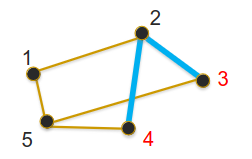
\includegraphics[width=80mm, scale=0.5]{bfs-esempio-pesi.png}
\end{center}
In poche parole è come se ogni arco avesse peso 1.
\subsection*{BFS(G,s) - Visita in ampiezza}
Significa effettuare la visita di un grafo \textbf{non} orientato G, a partire da un vertice
sorgente s:
\begin{itemize}
    \item All'inizio viene visitata la sorgente s
    \item Vengono poi visitati uno dopo l'altro tutti gli adiacenti di S
    \item In seguito, per ogni adiacente v di s, vengono visitati uno dopo l'altro
    gli adiacenti di v non ancora visitati
    \item Si prosegue a visitare gli adiacenti degli adiacenti e via di seguito
\end{itemize}
Tradotto in un esempio pratico:
\begin{itemize}
    \item Viene visitato s
    \item Vengono visitati tutti i vertici a distanza 1 da s
    \item Vengono visitati tutti i vertici a distanza 2 da s
    \item Vengono visitati tutti i vertici a distanza 3 da s
    \item etc.
\end{itemize}
\subsection{Caratteristiche di BFS}
\begin{itemize}
    \item Visita tutti e i soli vertici raggiungibili da s (vedremo che per DFS non sarà così)
    \item Ogni vertice del grafo viene visitato al più una volta
    \item Permette di trovare la distanza (in archi) da s di tutti i vertici
    raggiungibili dalla sorgente
\end{itemize}
\section{Colore Vertici}
I vertici hanno associato un colore:
\begin{itemize}
    \item vertice \underline{bianco} \ra vertice non visitato
    \item vertice \underline{grigio} \ra vertice visitato (adiacenti non
    completamente visitati)
    \item vertice \underline{nero} \ra vertice visitato (adiacenti completamente visitati)
\end{itemize}
%Slide 19 BFS